\documentclass{VUMIFPSkursinis}
\usepackage{algorithmicx}
\usepackage{algorithm}
\usepackage{algpseudocode}
\usepackage{amsfonts}
\usepackage{amsmath}
\usepackage{bm}
\usepackage{caption}
\usepackage{color}
\usepackage{float}
\usepackage{graphicx}
\usepackage{listings}
\usepackage{subfig}
\usepackage{wrapfig}

% Titulinio aprašas
\university{Vilniaus universitetas}
\faculty{Matematikos ir informatikos fakultetas}
\department{Programų sistemų katedra}
\papertype{Programų kūrimo proceso laboratorinis darbas}
\title{Įmonės ,,Mėnuliukai technologies" programų kūrimo proceso aprašas (Pirmas laboratorinis darbas)}
\titleineng{Description of the development process of the ,,Moon technologies" company ("First laboratory work")}
\status{4 kurso 3 grupės studentai}
\author{Matas Savickis, Justas Tvarijonas, Džiugas Mažulis}
\secondauthor{Greta Pyrantaitė, Andrius Bentkus}


\supervisor{Saulius Ragaišis, Doc., Dr.}
\date{Vilnius – \the\year}

% Nustatymai
% \setmainfont{Palemonas}   % Pakeisti teksto šriftą į Palemonas (turi būti įdiegtas sistemoje)
\bibliography{bibliografija}

\begin{document}
\maketitle

\tableofcontents

\sectionnonum{Įvadas}
\section{Kūrimo procesas}

	\begin{figure}[H]
	\centering
	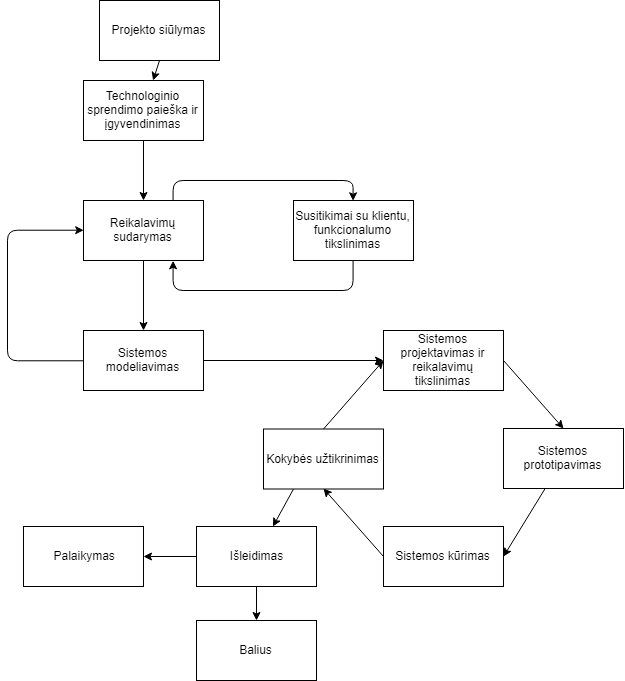
\includegraphics[scale=0.7]{img/SoftwareProcessMoonTechnologies}
	\caption{Sistemos kūrimo procesas} % Antraštė įterpiama po paveikslėlio
	\label{img:mlp}
	\end{figure}

	\subsection{Projekto siūlymas}
	\subsection{Technologinio sprendimo paieška ir įgyvendinimas}
	\subsection{Reikalavimų ciklas}
		\subsubsection{Reikalavimų sudarymas}
		\subsubsection{Susitikimai su klientu, funcionalumo tikslinimas}
	\subsection{Sistemos maketas}
	\subsection{Sistemos projektavimas}
	\subsection{Sistemos prototipavimas}
	\subsection{Sistemos kūrimas}
	\subsection{Kokybės užtikrinimas}
	\subsection{Išleidimas}
	\subsection{Palaikymas}
	\subsection{Balius}
	



\sectionnonum{Rezultatai ir išvados}




\end{document}
